%The background should set the project into context by motivating the subject matter and relating it to existing published work. The background will include a critical evaluation of the existing literature in the area in which your project work is based and should lead the reader to understand how your work is motivated by and related to existing work.
\chapter{Background research}
This chapter aims to introduce some concepts surrounding our problem domain, which to help the reader to understand and follow easier the following more technical chapters. I also present a review of the related work that has been done in this area. The below sections look at some of the key aspects and problems that arise. I then conclude by providing a number of alternative methods for solving our problem.

%Explain Curtailments (short turning) - reasons for this are: delays, planned roadworks or events, insufficient layover, improve overall realiability of the service fill gaps, prevent breaches - drivers hours regulation
%Bus bunching 
\section{London Bus Network}
London bus network is one of the most advanced and renowned in the world. It runs 24 hours and it is extensive and frequent. Every route in the network is tendered to different bus company operator \cite{busTendering}. These operators agree with TFL that the routes they are operating would be served either according to a predefined fixed schedule (e.g. a bus stop need to be served at 1pm, 3pm etc.)or on a headway (e.g. a bus stop need to be served every 5 minutes). However under different circumstances some delays occurring on a given route are beyond the control of the different bus operator companies. A simple example could be a burst water/gas pipe on a street used by a bus route or any other incident (even terrorist attacks \cite{centreComm}) and even simply a severe congestion. In situations like this bus operators have no authority or power to overcome such problems on their own. They can only ask CentreComm to intervene. CentreComm can do so by for example implementing a short/long term diversions or curtailments (short turning) some of the buses on the affected routes.

Buses in the network can be classified by multiple factors, however for the purpose of this report the main distinction we need to consider are high and low frequency bus routes. High frequency routes are routes where there are 5 or more buses per hour attending a given bus stop. Low frequency routes are those that have 4 or less buses alighting at a stop.
\section{CentreComm}
CentreComm is TFL's emergency command and control room responsible for all public buses in London. It is has been in operation for more than 30 years \cite{centreComm} and it employs a dedicated
team of professionals who work 24 hours 364 days in the year. They are dealing with more than a 1000 calls on a daily basis. The majority of these calls come from bus drivers or bus company operators regarding problems and incidents happening within the bus network. CentreComm staff implement planned long and short term changes in the bus network in response to different events taking place in the capital (including the 2012 Olympics). They are also responsible for reacting in real time to any unexpected and unpredicted changes and disruptions, maintaining the smooth, reliable and sage operation of London busy bus network.

London bus network consists of around 680 bus routes operated by more than 8000 buses \cite{glads}. Each of this buses is equipped with state of the art iBus system to help monitor and manage this enormous fleet. CentreComm's way of operation has been transformed beyond recognition since it has first opened and today. It started more than 30 years ago \cite{centreComm} and it consisted of a couple of operators equipped with two way radios and pen and papers. Today CentreComm operators make use of numerous screens each displaying interactive maps (displaying each bus location) and CCTV cameras in real-time. However there is still a lot of room for automation and improvement in their way of operation in order to effectively and efficiently maintain the growing bus network.

%CentreComm is not responsible for the fleet management as mentioned above. The emergency control and command room comes into place when there are planned or unplanned events affecting the bus network which need to be taken care of. They are responsible in assisting the bus drivers and bus company operators to manage their schedules when there are events which are beyond their control.
%CentreComm is not responsible for the fleet management as this is contracted to the bus operators which are responsible for maintaining reliable service according to agreed contracts. The emergency control room comes in place when there are planned or unplanned events which disrupt the transport network. They are also responsible for helping the bus operators once they cannot maintain the service they are responsible for due to traffic congestion or other issues which are beyond their control. However currently CentreComm relies on the bus drivers and bus operators for letting them know of such cases as they do not have a system which to signal them about these issues. All the information they need is there and they have access to it however they do not have the resources to manually monitor each of the 8000+ buses.
\section{iBus AVL}
Automatic vehicle location systems make use of the Global Positioning System (GPS) to enable the remote (using the internet) tracking of the locations of the vehicles in a given fleet. This system combines a number of technologies including GPS, cellular communications and more with the goal of improving and cutting the cost of fleet management. 

All of London buses operating on the TFL bus network have been equipped with state of the art and award wining \cite{ibusAward} AVL system named iBus \cite{ibus}. This system has opened a range of new applications that could be built on top of it using the information that is made available. The iBus system consist of a number of computer and communication systems, sensors and transmitters as described in \cite{Hounsell201276} and \cite{eps354267}.
One of the key components of the system on-board unit (OBU) which mounted on each of
buses in the TFL bus fleet and consists of a computational unit connected to
sensors and GPS transmitters (see figure 1 below taken from \cite{Hounsell201276}). 
\begin{figure}[ht!]
\centering
	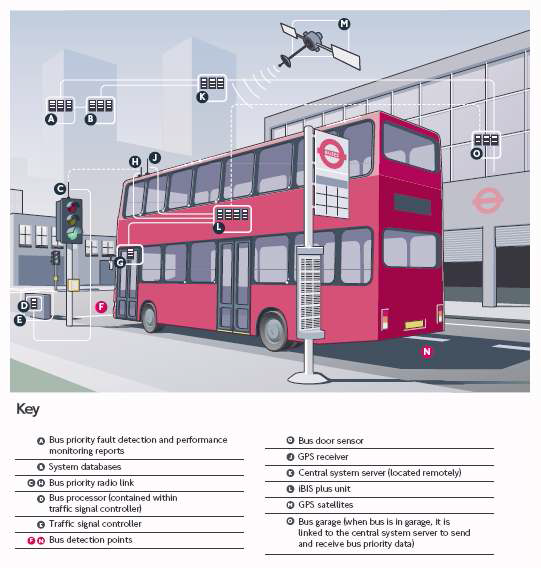
\includegraphics[scale=0.8]{Figures/iBus.png}
\caption{Overview of iBus System (Source: Transport for London, 2006a) \label{overflow}}
\end{figure}
This OBU is responsible for a number of tasks including a regular (approximately every 30 seconds) transmission of the bus location. This information is currently used by the different bus operators for fleet management as well as by CentreComm for real-time monitoring of the buses and their locations. There are have been a number of other applications and systems that have been implemented and put in to use as a result of the data that is generated by the iBus AVL. Some examples include Countdown (real-time passenger information), improved bus priority at traffic signals and more \cite{Hounsell201276}. This has led to improved and more affordable transport service.

CentreComm operators have access to an online system showing each bus location in the network on a map in real-time. This system allows them to see whether a given bus is behind, ahead or on time according to its schedule. However this does not show or alert the control room staff if a bus or a route is disrupted. Control room staff also can see when was a given bus expected to arrive at a given bus stop and when it actually arrived, but this again is only per individual bus. Currently the work-flow is such that CentreComm need to go and analyse all this information manually (once bus drivers or bus company operator have contacted/alerted the control room) in order to figure out if a there is a problem and how severe it is. This is very inefficient, tedious and error prone process. Here is where our project comes into place to address the lack of preprocessed information.

\section{Related Work}
The main problem posed by this project of detecting disruptions in the bus network can be also translated to short term traffic congestion detection. This is valid as we are not interested in individual bus delays. Some examples of such single instances of bus disruptions are customer incident on board of a single bus or technical fault with this bus etc. We are interested into finding routes/sections in the network which are delay/disrupted and this beyond the control of individual bus operators. Most often such problems are due some sort of congestion or road closures/repairs. However road problems are in most cases linked with increased traffic congestions as roads are used by other vehicles as well.

The literature is full of research towards accurately predicting bus arrival times with various computational models being used \cite{altinkaya2013urban}. Also there is a lot of work done toward detecting calculating travel times in non urban environment. This include approached based on AVL probe data and automatic vehicle identification (AVI) as well as induction loops \cite{Vlahogianni20143}. There are also plenty research done towards traffic congestion detection based on AVL probe data \cite{Vlahogianni20143}. However there are significant challenges due to the nature of the urban environment it self. Densely populate areas are influenced by many factors which could be affecting the general traffic flow. Another problem posed by urban environments is the irregularity of the AVL data transmission because of for example weak or lost signal at times (e.g. due to high buildings) or even there could be some noise which reduces the accuracy of the stated location. 

There is however little research to my knowledge which focusses on the issues of detecting and short-term forecasting of traffic congestion/disruptions in arterial urban environment  \cite{Vlahogianni20143} \cite{5625144}. As it can be seen from the tables in figures A.1 to A.4 taken from \cite{Vlahogianni20143}. From these tables we can easily see that most of the that has been done has focussed on motorways and also has employed data from static detector points (e.g automatic vehicle identification). Only in recent years we can see that more attention has been given to the use of GPS and AVL data. This is probably due to increased popularity and mass usage of such technologies. The literature is abundant of research on addressing the issues of bus prioritisation at traffic signals and junctions \cite{eps52676} and \cite{clarke2007}, but this is not directly related to our problem domain and thus is not discussed further in this report.

%For this reason in order to address our problem domain however we are not interested specifically in the general congestion as this could for example not affect the operation of the TFL bus fleet directly. A simple reason for this could be because there are significant amount of street which have a designated bus lanes which are prohibited for use by the general traffic. However there are studies showing that even under such circumstances there is a correlation between the general traffic flow and the performance of the buses in the same network [REFERENCE]. For our project we are interested however only in detecting the disrupted routes (sections of routes) and the severity of the disruption in the TFL bus network. We are interested in monitoring and detecting delays that are occurring in the network which would be classified, beyond the control of individual bus operator, by CentreComm.

%The literature review that has been undertaken as part of this project has showed that there are multiple approaches that could be undertaken to solve the problem posed by this project. There could be found different classifications of the models for predicting bus travel time\cite{surveyAIApplications}. According to \cite{urbanBusArrivalTimeCompModels} we could classify them into four computational models:
%\begin{itemize}
%	\item Based on historical data
%	\item Statistical 
%	\item Kalman Filtering 
%	\item Machine Learning
%\end{itemize}
%We could also add hybrid model which takes a combinational from the above [REFERENCE].

The approaches and research that we have examined show us that the the main model that have been used for detecting and forecasting short-term traffic congestion/disruptions are:
According to \cite{youKim} traffic forecasting models could be categorised as follows:
\begin{itemize}
	\item Statistical models
	\item Computer Simulations
	\item Mathematical Optimisation
	\item Artificial Intelligence
\end{itemize}
The statistical models could be further subdivided to:
\begin{itemize}
	\item Historical
	\item Time Series
	\item Nonparametric regression
	\item Hybrid
\end{itemize}
From the above the most widely used and well defined are the statistical models. From them the historical approaches are relatively easy for implementation and have fast execution speed, but have difficulty with dealing with incidents. Time series models have many applications and are well formulated. Because of their wide usage and advantages and the available AVL data for this project
we focus our attention on time series analysis for the rest of this report.

\section{Time Series}
Time series is a sequence of data readings taken during successive time intervals. This could be a continuous recording of readings or a set of discrete readings. In the context of our project we have the continuous process of bus readings (generated by the AVL system) being generated and transmitted. Analysis of time series data could be performed in order to extract and calculate some meaningful statistics from the data \cite{shumway2010time}. This could also result in producing a forecast of the data of interest for the next (future/unobserved) period of time based on the past observations. In order to highlight trends and make predictions we need to employ time series analysis techniques. Below I have presented some of the available techniques that could be employed when analysing time series data. It is not an exhaustive review of all available methods and models as I have tried to keep the discussion relevant to this project.

%Time series analysis is performed on time series data in order to extract some meaningful statistics from the data. In addition to the time series analysis time series forecasting could also be performed to come up with a prediction for the next period in time based on what has been observed in the past. In our problem this would mean having a number of bus readings we could analyse them and come up with prediction of what would be state in the next point in time. There also different smoothing techniques which would remove random abnormal fluctuation (e.g. an incident with a single bus).In the below sections we look at a number of different approaches to analysing and forecasting the next state of the network from the available data in real-time (we update our forecast whenever more data becomes available).

\subsection{Moving Averages}
Moving average also called rolling or running average is a statistical calculation method. It is universal analysis technique. It is type of mathematical convolution \cite{shumway2010time}. It helps to analyse data series by calculating a series of averages of subsets of the data. It can also be referred to as rolling or moving mean and it acts like a filter. Moving averages is commonly used in time series data analysis. It can be used in order to smooth out  a time series data with the aim of highlighting or estimating the underlying trend of the data. The other main usage is as a forecasting method again for time series. The main strength of these methods is that they are easy to understand.  Moving averages are often used as the building block for more complex time series analysis. Below are the three main type of moving averages.

\subsubsection{Simple Moving Average}
Simple moving average (SMA) is calculated by adding all the observations for a given period of time and dividing this sum by the number of observations. This is popular statistical technique which is mainly used to calculate the trend direction. The simple average is only useful for estimating the next forecast when the data does not contain any trends. Each observation is weighted equally. If we consider shorter term averages they would react quicker to changes while long term averages would have greater lag. The equation for calculating SMA is given below as equation 2.1.\\

\begin{equation}\label{sma}
	SMA = \frac{\sum_{0\le i\le n}\textrm{Value(i)}}{n}
\end{equation}

\subsubsection{Weighted Moving Average}
The problem with the simple moving average is that it weighted all data points equally. Meaning that both older and newer data would have the same effect on the average. This however is not the case when using weighted moving average (WMA). In WMA model each data point would be weighted differently according to when the observation was made. For example if we consider a n period moving average we could multiply the oldest observation by \[\frac{2*1}{n(n+1)}\] and the newest by \[\frac{2*n}{n(n+1)}\]. This would mean that recent data have bigger impact on the result. It is important that the weights add up to 1. The general equation for calculating WMA is given below as equation 2.2.

\begin{equation}\label{wma}
WMA = \frac{\sum_{0\le i\le n}(\textrm{Weight(i)}\textrm{Value(i)})}{\sum_{0\le i\le n}Weight(i)}
\end{equation}

\subsubsection{Exponential Moving Average}
Exponential smoothing was first suggested by Robert Goodell Brown \cite{FOR3980040103}. 
%Exponential Smoothing for Predicting Demand. Cambridge, Massachusetts: Arthur D. Little Inc. p. 15.] and then expanded by Charles C. Holt in 1957.[Holt, Charles C. (1957). "Forecasting Trends and Seasonal by Exponentially Weighted Averages". Office of Naval Research Memorandum 52. reprinted in Holt, Charles C. (January–March 2004). "Forecasting Trends and Seasonal by Exponentially Weighted Averages". International Journal of Forecasting 20 (1): 5–10. doi:10.1016]

Exponential moving average (EMA) or also called exponential smoothing is very similar to WMA. The main difference is that in order to calculate it we do not need to keep all the data, but we could only store the latest value and the previous forecast only. Exponential moving average weights the data points exponential which means that the oldest data would have minimalistic effect on the result.There exist few exponential smoothing techniques including single, double and triple exponential moving average. Equations 2.3 and 2.4 give the simplest form for calculating single exponential smoothing. In this equation $\alpha$ is called the smoothing factor and it is usually a value between 0 and 1. The closer $\alpha$ is to 0 have greater smoothing factor, but are less responsive to recent changes thus have greater lag. Values of $\alpha$ that are near to 1 have less smoothing effect, but are very reactive to recent changes in the data. 

\begin{align}\label{ema}
EMA_1 = Value_1 \\
\textrm{for } t > 1\textrm{, }EMA_t = \alpha Value_t + (1-\alpha) EMA_{t-1}
\end{align}

\subsubsection{Summary}
If we compare the three types (simple, exponential and weighted) we can clearly see that the simple moving average offers the most smoothing however there is the trade-off of the biggest lag.The exponential moving average will react faster to changes and sits closer to the actual readings, however it might overreach at times. The weighted moving follows the movement even more closely than the exponential moving average. Determining which one to use depends on the objective. If a trend indication with better smoothing and little reaction for shorter movements then the simple average should produce the best results. However if smoothing is desired where you can still see shorter movements then it is better to use either WMA or EMA.

\subsection{Peak Detection}
Detection and analysis of peaks (spikes) and valleys in time series is important in many applications (e.g signal processing, bioinformatics and many more). Peaks and valleys usually represent either significant events or errors in time series data. In our domain we are mostly interested in detecting high sudden changes in the traffic congestion conditions (e.g along route/sections in the bus network). Peaks could be easily identified by visualising the data, however we are interested in automating this process. In the literature has many examples of peak detection application one such for example is \cite{simplePeakDetection} used for spike detection in microarray data (anther example could be found in \cite{Azami2014491}). We do not go into details of any particular algorithms here because of the time constraints of this project (a study peak detection algorithms could be found in \cite{ventzas2011peak}). However it is worth to note that spike detection and analysis could be used to classify events that are detected. A simple example could be to distinguish if given detected congestion/disruption is incident related (e.g. sudden) or it is general traffic jam (e.g. rush hour).

\section{Other}
Other approaches that have could be used include Kalman filtering \cite{kalmanFiltering} \cite{Guo201450}, Markov Chains \cite{Qi201495} \cite{Ramezani20121576}, Machine learning \cite{herring2010real}, Bayesian networks \cite{Wang201479}. 

%In this report we do not go into further details of these alternative  as the aim of the project is to fully understand the requirements of the CentreComm and propose a prototype which to serve as a proof of concept.

%Markov chain is a stochastic process that transitions from one state to another using some state space. It is characterised by the property of having no memory. This means that the next state depends only on the current state and not on the preceding sequence of state transitions. This is called a Markov property.

%Markov chains are usually used in modelling many practical problems. They are also effective in modelling time series. In this paper, we apply the Markov chains model to analyse and predict the time series. Some series can be expressed by a first-order discrete-time Markov chain and others must be expressed by a higher order Markov chain model. Numerical examples are given. The results show that the performance and effectiveness of the Markov chain model to predict the time series is very well.[TAKEN FROM - Application of Markov Chains to Analyze and Predict the Time Series]

\section{Summary}
In this chapter I have aimed to provide the reader with broad view of the background of our problem and its domain. Detailed overview of the operations and the technologies and work flows used by TFL's bus command and control centre has been provided. This has led to detailed review and discussion of the related work that has been found in the literature. The chapter concluded with discussion on some of the available approaches. The exact approach taken and any implementation details are described in detail in Chapter 5 along with presentation and discussion of the data that has been provided by TFL for this project.